\documentclass{article}
\usepackage[utf8]{inputenc}
\usepackage[spanish,es-nodecimaldot,es-tabla]{babel}
\usepackage{amsmath}
\usepackage{graphicx}
\usepackage[colorlinks=true, allcolors=blue]{hyperref}
\usepackage[makeroom]{cancel}
% hyperref para autoref, amsmath para split
\usepackage{subfig,placeins}
\usepackage{libertine}
\usepackage[libertine]{newtxmath}
\graphicspath{{./figs/}{./imgs/}}
\usepackage[font=small,labelfont=bf]{caption}
\usepackage{listings,figs/tuneatantito}
\newcommand\pder[2]{\ensuremath {\dfrac{\partial#1}{\partial#2}}} 
\newcommand{\ppder}[2]{ \ensuremath {\dfrac{\partial^2 #1}{\partial #2^2}}}
\newcommand{\ppcder}[3]{ \ensuremath {\dfrac{\partial^2 #1}{\partial #2\partial #3}}}

\title{E2}
\author{Pedraza-Espitia S\href{https://pedraza-espitia.github.io/modnum}{.}}
\date{}

\begin{document}

\maketitle

\section{Esquema de discretización estable para la ecuación de advección}
El código siguiente y la \autoref{fig:e2i4} muestran como con la condición CFL igual a 1 el esquema se mantiene estable, pero aumentando Del\_T a 2.1 el esquema se vuelve inestable, esto es porque $c\Delta t/\Delta x = 2.1 > 1$
\lstinputlisting[language=Matlab]{./MatlabCodes/E2_i4.m}
%%%%%
\begin{figure}[!ht]
\centering
  \hfill\subfloat[]{
  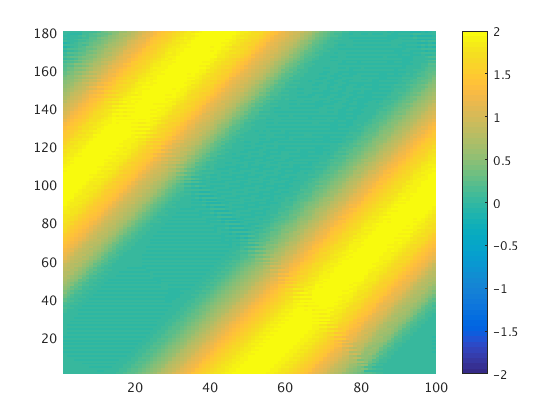
\includegraphics[width=0.35\textwidth]{e2estable}
  }\hfill
  \subfloat[]{%\label{fig:}
  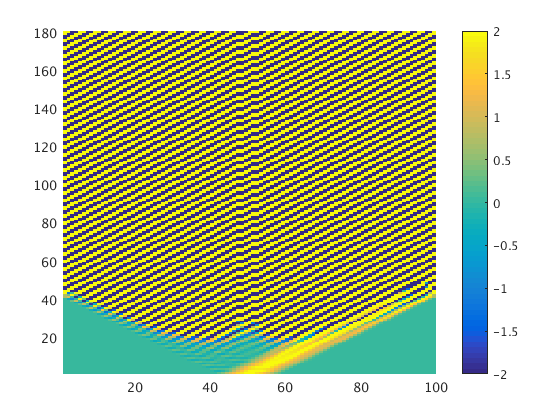
\includegraphics[width=0.35\textwidth]{e2inestable}
  }\hfill
  \caption{Gráficas (a) estable e (b) inestable.}%
\label{fig:e2i4}
\end{figure}
%%%%%

\section{Utilizando el criterio de von Neumann}
\begin{equation}
	\frac{u_j^{n+1}-u_j^{n-1}}{2\Delta t} + c \frac{u_{j+1}^{n}-u_{j-1}^{n}}{2\Delta x} = 0
	\label{eq:adveccion}
\end{equation}

La solución analítica es
\begin{equation}
	u = u_0 e^{ik(x - c t)}
\end{equation}

La solución numérica es
\begin{equation}
	u_{j}^{n} = u_0 e^{ik(j\Delta x - c_D n \Delta t)}
	\label{eq:solnumerica}
\end{equation}

Vamos a desarrollar los términos en \eqref{eq:adveccion} con la ayuda de la \autoref{eq:solnumerica}
\begin{equation}
	\begin{split}
	u_{j}^{n+1} = & u_0 e^{ik(j\Delta x - c_D (n+1) \Delta t)} \\
		=& u_0 e^{ik(j\Delta x - c_D n\Delta t - c_D\Delta t)} \\
		=& u_{j}^{n} e^{-ik c_D\Delta t} \\
	\end{split}
\end{equation}

definiendo $
	\lambda \equiv e^{-ik c_D\Delta t}
$

\begin{equation}
	u_{j}^{n+1} = u_{j}^{n} \lambda
\end{equation}

\begin{equation}
	\begin{split}
	u_{j}^{n-1} = & u_0 e^{ik(j\Delta x - c_D (n-1) \Delta t)} \\
		=& u_0 e^{ik(j\Delta x - c_D n\Delta t + c_D\Delta t)} \\
		=& u_{j}^{n} e^{ik c_D\Delta t} \\
		=& u_{j}^{n} \lambda^{-1} \\
	\end{split}
\end{equation}

\begin{equation}
	\begin{split}
	u_{j+1}^{n} = & u_0 e^{ik((j+1)\Delta x - c_D n \Delta t)} \\
		=& u_0 e^{ik(j\Delta x - c_D n\Delta t +\Delta x)} \\
		=& u_{j}^{n} e^{ik \Delta x} \\
	\end{split}
\end{equation}

De la misma forma 
\begin{equation}
	\begin{split}
	u_{j-1}^{n} = & u_0 e^{ik((j-1)\Delta x - c_D n \Delta t)} \\
		= & u_0 e^{ik(j\Delta x - c_D n\Delta t - \Delta x)} \\
		= & u_{j}^{n} e^{-ik \Delta x} \\
	\end{split}
\end{equation}

Sustituimos los resultados en \autoref{eq:adveccion}
\begin{equation}
	\frac{u_j^{n}\lambda-u_j^{n}\lambda}{2\Delta t} + c \frac{u_{j}^{n}e^{ik \Delta x}-u_{j}^{n}e^{-ik \Delta x}}{2\Delta x} = 0
\end{equation}

multiplico por $\frac{2\lambda \Delta t}{u_j^n}$
\begin{equation}
	\lambda^2 -1 + c \Delta t \frac{\left( e^{ik \Delta x} - e^{-ik \Delta x} \right)}{\Delta x}= 0
\end{equation}

Usamos la identidad trigonométrica
\begin{equation}
	\lambda^2 + \frac{c\Delta t}{\Delta x} \left( 2i \sen(k\Delta x) \right)\lambda -1 = 0
\end{equation}

Resolvemos para $\lambda$
\begin{equation}
\begin{split}
	\lambda = & \frac{ \left[ -\frac{c\Delta t}{\Delta x}\left( 2i \sen(k\Delta x) \right) \right]  \pm \sqrt{ \left[ \frac{c\Delta t}{\Delta x}\left( 2i \sen(k\Delta x) \right) \right]^2 + 4}}{2}\\
	= & -i\frac{c\Delta t}{\Delta x} \sen(k\Delta x) \pm \sqrt{ 1 - \left[ \frac{c\Delta t}{\Delta x}\left( \sen(k\Delta x) \right) \right]^2}
\end{split}
\end{equation}

$\lambda$ es un número complejo, si calculamos su valor absoluto y consideramos que $\left[ \frac{c\Delta t}{\Delta x}\left( \sen(k\Delta x) \right) \right]^2 \leq 1$, entonces

\begin{equation}
	\left| \lambda \right|^2 =  \left[ \frac{c\Delta t}{\Delta x}\left( \sen(k\Delta x) \right) \right]^2 + 
	\left\{ \sqrt{ 1-  \left[ \frac{c\Delta t}{\Delta x}\left( \sen(k\Delta x) \right) \right]^2 } \right\}^2 = 1
	\label{eq:valabscuadlambda}
\end{equation}

Si \autoref{eq:valabscuadlambda} se cumple:
\begin{equation}
	\frac{c\Delta t}{\Delta x}\left| \sen(k\Delta x) \right| \leq 1
\end{equation}

y debido a que $| \sen(k\Delta x)| \leq 1$ $\Rightarrow$ Obtenemos la condición de estabilidad
\begin{equation}
	c \leq \frac{\Delta x}{\Delta t}
\end{equation}

o bien
\begin{equation}
	c  \frac{\Delta t}{\Delta x} \leq 1
\end{equation}

Ahora para entender que pasaría en el caso en que 
\begin{equation}
	 \left[ \frac{c\Delta t}{\Delta x}\left( \sen(k\Delta x) \right) \right] > 1
\end{equation}
definimos $\gamma \equiv \frac{c\Delta t}{\Delta x}\left( \sen(k\Delta x) \right)$, entonces $\gamma^2 > 1$, y

\begin{equation}
	\left| \lambda \right| = -i\gamma \pm i\sqrt{\gamma^2 - 1} = i \left( -\gamma \pm \sqrt{\gamma^2 - 1} \right)
\end{equation}
\begin{equation}
	\left| \lambda \right|^2 = \left( -\gamma \pm \sqrt{\gamma^2 -1} \right)^2 = \gamma^2 \pm 2\gamma\sqrt{\gamma^2 -1} + \gamma^2-1
	\label{eq:unaraizm1}
\end{equation}
la ec \eqref{eq:unaraizm1} tiene al menos un raiz mayor que 1, por tanto $c > \Delta x / \Delta t$ y en este caso $|\lambda| > 1$, \textit{i.e. } es inestable.


\end{document}